
\section{Einphasiger Wechselrichter}
    \begin{tabu}{|l|l|p{0.3\textwidth}}
        \cline{1-2}
        Schaltzeitpunkte 
        &\ $\begin{aligned}
        T &= \frac{1}{f}, \quad dt = \frac{T}{N-1}\\
        t_e(i) &= (i-1) \cdot dt\\
        t_a(i) &= t_e(i) + k \cdot dt \cdot |\sin(\omega \cdot t_e(i))|
        \end{aligned}$ 
        & \multirow{2}{*}{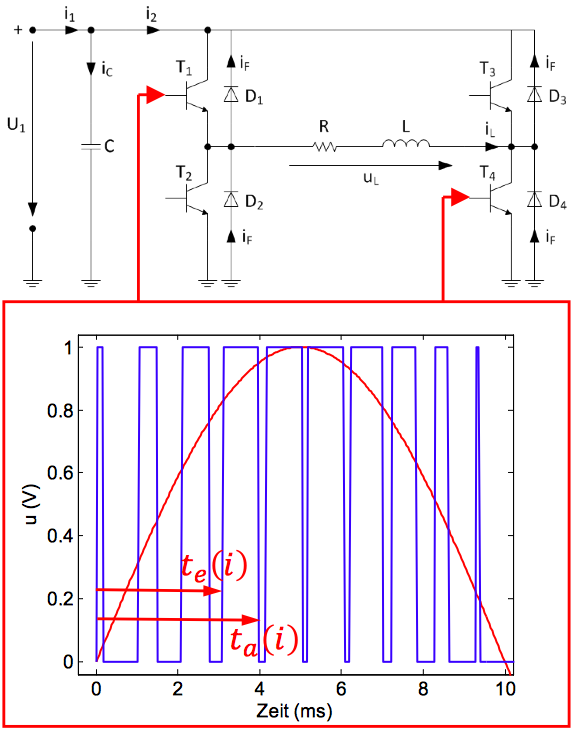
\includegraphics[width = 0.9\linewidth]{./pictures/wechselrichterEinphasig.png}}\\
        \cline{1-2}
        Laststrom 
        &\ $\begin{aligned}
        \tau &= \frac{L}{R}\\
        t &\in [t_{ei},t_{ai}]\\
        i_L(t) &= \frac{U_1}{R} \cdot \left( 1-e^{\frac{t_{ei}-t}{\tau}}\right) + i_L(t_{ei}) \cdot e^{\frac{t_{ei}-t}{\tau}}\\
        t &\in [t_{ai},t_{ei+1}]\\
        i_L(t) &= i_L(t_{ai}) \cdot e^{\frac{t_{ai}-t}{\tau}}
        \end{aligned}$ &\\
        \cline{1-2}
    \end{tabu}
    \\\\